\documentclass[12pt,a4paper]{report}

\usepackage[left=2cm, right=2cm, top=5cm]{geometry}
\usepackage{enumitem}
\usepackage{fontspec}
\usepackage{tikz}
\usepackage{amsmath}

\usepackage{algpseudocode}
\algblockdefx[Initially]{Initially}{EndInitially}{\textbf{initially do}}{\textbf{end initially}}
\algblockdefx[Upon]{Upon}{EndUpon}[1]{\textbf{upon #1}}{\textbf{end upon}}
\algblockdefx[AsSoon]{AsSoon}{EndAsSoon}[1]{\textbf{as soon as #1}}{\textbf{end as soon}}

\usetikzlibrary{graphs, shapes, graphdrawing}
\usegdlibrary{layered, force}

\begin{document}

	\newcommand{\upon}[1]{\textbf{Upon} #1 \textbf{do}}

	\begin{titlepage}
		\centering
		{\scshape\LARGE Universidad Nacional Autónoma de México \par}
		\vspace{1cm}
		{\scshape\Large Computación Distribuida\par}
		\vspace{1.5cm}
		{\huge\bfseries Tarea 6\par}
		\vspace{.5cm}
		{\Large\itshape Edgar Quiroz Castañeda \par}
	    \vspace{.5cm}
		{\Large\itshape Jerónimo Almeida Rodríguez \par}
		\vfill
		 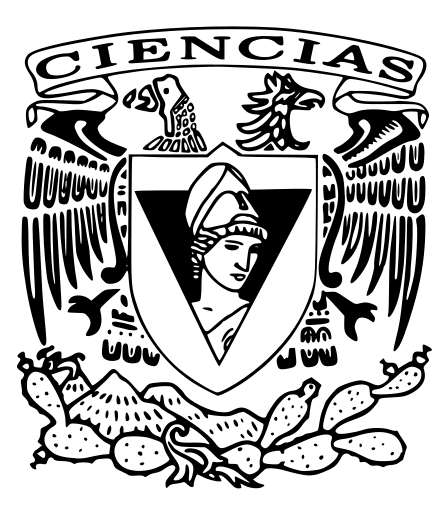
\includegraphics[width=0.5\textwidth]{escudo_f-ciencias.png}
		\vfill

		{\large Jueves 1 de octubre del 2018 \par}
	\end{titlepage}

	\pagebreak
	\setlength{\voffset}{-0.75in}
	\setlength{\headsep}{5pt}

	\begin{enumerate}
		\item {
			Sea $G = (V, E)$ una gráfica. Diseña un algoritmo $BFS$ basado en correr
			$|V|$ instancias del algoritmo $PIF$ cuya complejidad ser
			$O(|E|+|V|\cdot Diam(G))$ en mensajes y $O(Diam(G)^2)$ en tiempo.

			La idea de este algoritmo es recorrer la gráfica por capas por medio de
			una ejecución del $PIF$ por capa.\\
			Cada ejecución tiene el propósito de tomar el árbol de la ejecución
			anterior y agregarle todos los nodos a distancia una más que la ejecución
			anterior.\\
			Para hacer esto, el mensaje que se envía para decubrir son los valores de
			la distancia acumulada y el límite de distancia para esa ejecución en
			particular.\\
			Igualmente que en el otro $BFS$ distribuido, se actualiza la distancia a
			uno más de lo recibido si eso es mejor o igual a lo actual.\\
			Pero sólo se envía esa información a los vecinos en caso de que ellos
			aun estén en el alcance de la ejecución.\\
			Además, si no se es una de las hojas del árbol de la ejecución anterior,
			ni siquiera se envía a todos los vecinos, si no a todos los hijos, que ya
			se conocen desde al menos la ejecución anterior.\\
			En el caso de las hojas del árbol final o de los nodos intermedios del
			árbol de una ejecución dada, se envía la confirmación en cuanto se tiene
			la información de todos los vecinos, .\\
			Para las hojas del árbol de la ejecución, se envía la confirmación en
			cuanto se entera de que es el límite del alcance de esa ejecución.\\
			Como confirmación se envía el conjunto de nodos en su subárbol.\\
			Cuando esto llega a la raíz, es el conjunto de todos los nodos que ya son parte
			del árbol.\\
			Si aun faltan nodos, entonces se aumenta el alcance y se inicia
			una nueva ejecución del $PIF$.
			Si se tiene a todos los nodos en el árbol, entonces el algorítmo acaba.

			\begin{algorithmic}[1]
				\Initially
					\State $children \gets \emptyset$
					\State $acks \gets \emptyset$
					\State $nacks \gets \emptyset$
					\State $discovered \gets \emptyset$
					\If{$p_{id} = root$}
						\State $distance \gets 0$
						\State $parent \gets p_{id}$
						\State $currentBound \gets 1$
						\State send $(distance, currentBound)$ to $neighbors$
					\Else
						\State $parent \gets \bot$
						\State $distance \gets \infty$
					\EndIf
				\EndInitially
				\Statex

				\Upon{receiving $(distance_p, bound)$ from $p$}
					\If{$distance_p + 1 \leq distance$}
						\State $parent \gets p$
						\State $distance \gets distance_p + 1$
					\Else
						\State send $nack$ to $p$
					\EndIf
					\If{$distance -1 < bound $}
						\State send $(distance, bound)$ to $children$
					\ElsIf{$distance -1 = bound $}
						\State send $(distance, bound)$ to $neighbors \setminus \{p\}$
					\ElsIf{$distance = bound$}
						\State send $(ack, discovered)$ to $p$
					\EndIf
				\EndUpon
				\Statex

				\Upon{receiving $(ack, discovered_p)$ from $p$}
					\State $discovered = discovered \cup discovered_p$
					\State $acks = acks \cup \{p\}$
					\State $children = children \cup \{p\}$
				\EndUpon
				\Statex

				\Upon{receiving $nack$ from $p$}
					\State $nacks \gets nacks \cup \{p\}$
				\EndUpon
				\Statex

				\AsSoon{$acks \cup nack = neighbors$}
					\State $acks \gets \emptyset$
					\If{$p_{id} = root$}
						\If{$discovered = V$}
							\State return
						\EndIf
						\If{$acks = children$}
							\State $currentBound \gets currentBound + 1$
							\State send $(distance, currentBound)$ to $neighbors$
						\EndIf
					\Else
						\State send $(ack, discovered)$ to $parent$
					\EndIf
				\EndAsSoon
			\end{algorithmic}
			Con un tiempo normalizado, se tiene que el tiempo para llegar a el nodo $v$
			que está a distancia del diámetro es
			\begin{align*}
				2+4+6+8+...+2\cdot Diam(G) &= 2 (1+2+3+4+...+Diam(G))\\
																	 &= 2\frac{Diam(G)(Diam(G)+1)}{2}\\
																	 &= Diam(G)(Diam(G)+1) \in O(Diam(G)^2)
			\end{align*}
			Pues la ronda $i$ tarda a lo más $2i$ unidades de tiempo, $i$ unidades
			para llegar a el nodo $i$ de la trayectoria de la raíz a $v$, y otras
			$i$ unidades para volver a la raíz.\\
			Este es el último nodo que es agregado al árbol, precisamente porque su
			distancia a la raíz es el diámetro en el peor caso. Entonces este algoritmo
			tiene complejidad en tiepo de $O(Diam(G)^2)$.\\
			En cuanto a la complejidad en mensajes, se tiene que en cada ejecución,
			las aristas que se recorren por primera vez son únicamente las que están
			en el nuevo alcance. Cada una de estas aristas recibe el mensaje con
			la distancia y con el alcance, y devuelve un $ack$ o un $nack$. Como esto
			sólo pasa en la ronda donde son descubiertas, entonces se envían
			$2|E|$ mensajes. Luego, para recorrer el resto de la gráfica hasta
			la raíz se utilizan las trayectorias ya definidas por el subárbol
			descubierto en ejecuciones anterior, que tiene a lo más $|V|-1$ aristas.
			Como este recorrido se hace en cada ejecución, y hay $Diam(G)$ ejecuciones,
			entonces el resto de los mensajes son $(|V|-1)(Diam(G))$.\\
			Entonces, hay a lo más $2|E| + (|V|-1)(Diam(G)) \in O(|E| + |V|Diam(G))$
			mensajes.\\
			Entonces, la complejidad en mensajes es $O(|E| + |V|Diam(G))$.
		}
		\item {
			Explicar por qué el algorítmo Awerbuch $DFS$ tiene complejidad de tiempo
			$O(V)$ ($4|V|-2$) y en mensajes $O(E)$ ($4|E|$). Presentar un ejemplo
			de ejecución en la siguiente gráfica

			\begin{center}
				\begin{tikzpicture}[node distance = 3cm]
					\begin{scope}[every node/.style = {circle, draw}]
						\node (p1) {$p_1$};
						\node (p2) [above right of = p1] {$p_2$};
						\node (p3) [right of = p2] {$p_3$};
						\node (p4) [below right of = p3] {$p_4$};
						\node (p5) [left of = p4] {$p_4$};
						\node (p6) [below right of = p1] {$p_6$};
					\end{scope}

					\path[-] (p1) edge (p2);
					\path[-] (p1) edge (p5);
					\path[-] (p1) edge (p6);

					\path[-] (p2) edge (p3);
					\path[-] (p2) edge (p4);

					\path[-] (p3) edge (p4);

					\path[-] (p4) edge (p5);
					\path[-] (p4) edge (p6);

					\path[-] (p5) edge (p6);
				\end{tikzpicture}
			\end{center}
		}
		\item {
			Ver el video y mediante una lista de puntos explicar las ideas que se
			exponon. Cada punto no debe tener más de un par de líneas.
			The Physics and Philosophy of Time - with Carlo Rovelli https://youtu.be/-6rWqJhDv7M
		}
	\end{enumerate}
\end{document}
